\lezione{13}{19.04.17}

\section{Variabili aleatorie indipendenti}
Dal concetto di indipendenza tra \emph{eventi} discende l'\emph{indipendenza tra variabili aleatorie}, che indica la condizione in cui gli eventi modellizzati dalle variabili non si influenzano l'un l'altro.
Enunceremo alcuni criteri per stabilire l'indipendenza, alcuni dei quali inizieranno a mostrare l'utilità del valore atteso al di là dell'essere un semplice indicatore a sé stante; verrà inoltre illustrata la possibilità di costruire variabili indipendenti a partire da variabili qualsiasi.
Grazie all'indipendenza si potrà iniziare a estendere la teoria precedente a \emph{prodotti cartesiani} tra domini, a cui corrispondono gli eventi nelle \emph{$\sigma$-algebre prodotto} e le relative probabilità, le \emph{leggi congiunte}, costruite a partire dalle \emph{leggi marginali} mediante l'importantissimo \emph{teorema di Fubini-Tonelli}.
Potremo presto iniziare a trattare i \emph{vettori aleatori}, variabili aleatorie multidimensionali.


\subsection{Indipendenza di variabili aleatorie}
\begin{defn}
  \index{indipendenza!di VA}
  Siano $\Dom$ spazio di probabilità, $(E, \Ec)$, $(F, \Fc)$ spazi misurabili, e $X:\Omega \to E$ e $ Y:\Omega \to F$ VA. \\
  $X$ e $Y$ si dicono \textbf{VA indipendenti} $(X \indep Y)$ se:
  $$\PP(X \in A, Y \in B )= \PP(X \in A) \ \PP(Y \in B)  \quad  \forall A \in \Ec \enspace  \forall B \in \Fc$$
 \end{defn}
Ciò significa che ogni evento $A$ che riguarda $X$ è indipendente da ogni evento $B$ che riguarda $Y$. In altre parole, le \emph{previsioni} di $X$ e $Y$ \emph{non si influenzano} l'una con l'altra.
\begin{nb}
  Lo stesso $\omega \in \Omega$ determina il valore sia di $X$ che di $Y$ perché $\Omega$ è il dominio comune delle due VA.
\end{nb}

\medskip
\begin{ese}
  Date due monete truccate con probabilità di ottenere testa $0<p<1$ siano $\Omega =   \left \{ c, t \right \}^2$, $\omega=(\omega_1, \omega_2)$, $\Ac = 2^\Omega$.
  Si considerino ora gli eventi:
  \begin{figure}[ht]
    \centering
    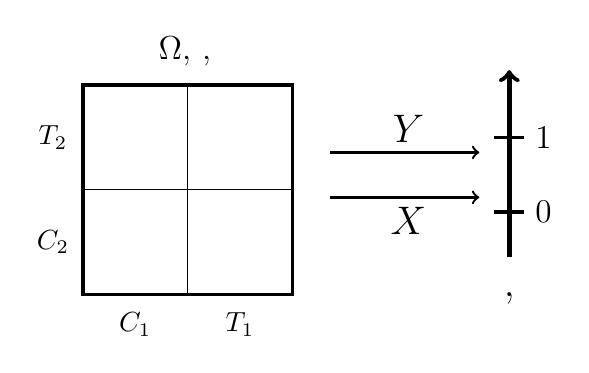
\begin{tikzpicture}[scale=0.95]
      \begin{scope}[shift={(-1.5cm,-1.5cm)}]
        \draw[scale=1.4] (0, 0) grid (2,2);
        \node at (0.7, -0.4) {$C_1$};
        \node at (2.1, -0.4) {$T_1$};
        \node at (-0.4, 0.7) {$C_2$};
        \node at (-0.4, 2.1) {$T_2$};
      \end{scope}
      \draw[very thick] (-1.5, -1.5) rectangle (1.3, 1.3);
      %Frecce
      \draw[->, line width=0.30mm] (1.8,0.4) node[above,xshift=1cm] {\Large $Y$} -- (3.8, 0.4);
      \draw[->, line width=0.30mm] (1.8,-0.2) node[below,xshift=1cm] {\Large $X$} -- (3.8, -0.2);
      \draw[->, line width=0.60mm] (4.2, -1) node[below, yshift=-.3cm] {\Large $\RR, \Bc$} -- (4.2, 1.5);
      %Tacchette
      \draw[line width=0.50mm] (4.4, .6) node[right] {\large $1$} -- (4, .6);
      \draw[line width=0.50mm] (4.4, -.4) node[right] {\large $0$} -- (4, -.4);
      %Scritte
      \node at (-.1, 1.75) {\large $\Omega, \, \Ac, \, \PP$};
    \end{tikzpicture}
    \caption{dominio e codominio della VAR}
    \label{dom-cod-var}
  \end{figure}
  \begin{itemize}
    \item $C_1 =$ croce sulla prima moneta = $\left \{ (c,c) , (c,t) \right \}=\left \{ \omega \in \Omega : \omega_1=c \right \} $
    \item $T_1 =$ testa sulla prima moneta = $C_1^C= \left \{\omega \in \Omega : \omega_1=t \right \} $
    \item $C_2 =$ croce sulla seconda moneta = $ \left \{\omega \in \Omega : \omega_2=c \right \} $
    \item $T_2= C_2^C$
  \end{itemize}
  Si sceglie $\PP$ tale che $\PP(T_1)=\PP(T_2)=p \enspace$ e $\enspace T_1 \indep T_2$. Di conseguenza, $T_1^C \indep T_2^C$.

  \needspace{3\baselineskip}
  Passando dal linguaggio degli eventi al linguaggio delle VA, si introducono due VA:\\[-4pt]
  $$X= \begin{cases} 1 & \text{se sulla prima moneta esce testa} \\ 0 & \text{se sulla prima moneta esce croce} \end{cases}$$
  $$\implies X:\Omega \to \RR \ \ \  (X=1)=T_1 \ \ \ (X=0)=C_1$$
  $$Y= \begin{cases} 1 & \text{se sulla seconda moneta esce testa} \\ 0 & \text{se sulla seconda moneta esce croce} \end{cases}$$
  $$\implies Y:\Omega \to \RR \ \ \ (Y=1)=T_2 \ \ \ (Y=0)=C_2$$
  Si può affermare che questo implica $X \indep Y$?

  Serve verificare che:
  $$\PP(X \in A, Y \in B)=\PP(X \in A) \ \PP( Y \in B) \quad \forall A,B \in \Bc $$
  L'uguaglianza è vera perché:
  \begin{itemize}
    \item se $A$ e $B$ contengono un solo valore, allora sono uguali a $T_1, T_2$ o i loro complementari ed essi sono indipendenti per costruzione;
    \item se $A$ o $B$ sono l'evento impossibile $\varnothing$, allora entrambi i membri sono nulli;
    \item se $A$ o $B$ sono l'evento certo $\Omega$, allora entrambi i membri sono uguali a 1.
  \end{itemize}

  Introduciamo ora le VA $Z=X+Y$ (numero di teste su due lanci), $W=X-Y$ e $V=\left | X-Y \right |$ (0 se i due risultati sono uguali, 1 altrimenti). \\
  $Z$ e $W$ non sono indipendenti? Per dimostrarlo ci servono due eventi le cui probabilità non si fattorizzano. Ad esempio, verifichiamo che $\PP(Z=2, W=1)\ne\PP(Z=2)\PP(W=1)$:
  \begin{itemize}
    \item $\PP(Z=2,W=1)=\PP(\varnothing)$, in quanto non abbiamo un'intersezione in cui si verificano entrambi gli eventi. Quindi $\PP(\varnothing)=0$;
    \item $\PP(Z=2)=\PP(X=1,Y=1)=p^2$;
    \item $\PP(W=1)=\PP(X=1,Y=0)=\PP(X=1)\PP(Y=0)=p(1-p)$.
  \end{itemize}
  Ma $p^3(1-p) \neq 0$ per $p$ non degeneri. Allora $\PP(Z=2, W=1)\ne\PP(Z=2)\PP(W=1)\enspace$ e $\enspace Z \centernot\indep W$. \\
  Si può dimostrare allo stesso modo che $Z \notindep V$; anzi, $V=h(Z)=Z(2-Z)$. Si noti che $X = f(Y)$ è l'opposto concettuale di $X \indep Y$.
\end{ese}

\subsection{Condizioni equivalenti}
\begin{teob}[\JPTh{10.1}]
  Siano $\Dom$ spazio di probabilità, $(E, \Ec)$ e $(F, \Fc) $ spazi misurabili. Siano inoltre le VA $X:\Omega \to E $ e $ Y:\Omega \to F $. Allora le seguenti affermazioni sono equivalenti:
  \begin{enumerate}
    \item $X \indep Y$;
    \item $ \PP(X \in A, Y \in B)=\PP(X \in A) \, \PP(Y \in B) \quad \forall A \in \Cc\enspace \forall B \in \Dc$ \\
    con $\Cc$ e $\Dc$ chiusi per intersezioni finite, $\Ec = \sigma(\Cc)$ e $\Fc = \sigma(\Dc)$;
    \item $ h(X) \indep g(Y) \ \ \forall h: (E, \Ec) \to (E', \Ec')$ misurabile e $\forall g: (F, \Fc) \to (F', \Fc')$ misurabile; \\*
    (se sono state definite bene, $h(X)$ non dà informazioni su $Y$ e $g(Y)$ non dà informazioni su $X$)
    \item $ \EE[h(X)g(Y)]=\EE[h(X)] \, \EE[g(Y)]$
    \begin{enumerate}
    \item $\forall h: (E, \Ec) \to (\RR,\Bc)$ misurabile e positiva, \\
        $\forall g: (F, \Fc) \to (\RR,\Bc)$ misurabile e positiva; \\
        (gli insiemi sono ben specifici e non possono essere scelti a caso)
    \item $\forall h: (E, \Ec) \to (\RR,\Bc)$ misurabile e limitata, \\
        $\forall g: (F, \Fc) \to (\RR,\Bc)$ misurabile e limitata; \\
        (le condizioni su $h$ e $g$ servono per l'esistenza dei vari integrali: $h$ dovrebbe essere $L^1$ della legge di $X$, ma visto che non ne sappiamo le specifiche usiamo le condizioni per accertarci che questo sia verificato)
    \item
      se $E, F$ sono spazi metrici e $ \Ec$, $\Fc$ le loro $\sigma$-algebre di Borel \\
      $\forall h: (E, \Ec) \to (\RR,\Bc)$ continua e positiva, \\
      $\forall g: (F, \Fc) \to (\RR,\Bc)$ continua e positiva; \\

    \end{enumerate}
  \end{enumerate}
\end{teob}

\smallskip
\needspace{3\baselineskip}
\begin{dimo}
  La dimostrazione si svolgerà così:
  \begin{figure}[H]
    \centering
    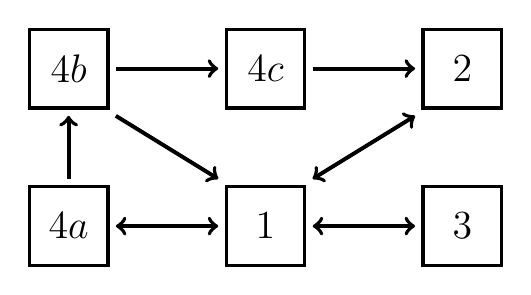
\begin{tikzpicture}
      %Rettangoli
      \draw[line width=0.40mm] (0,2) rectangle (1,3) node[pos=0.5] {\Large $4b$};
      \draw[line width=0.40mm] (0,0) rectangle (1,1) node[pos=0.5] {\Large $4a$};
      \draw[line width=0.40mm] (2.5,2) rectangle (3.5,3) node[pos=0.5] {\Large $4c$};
      \draw[line width=0.40mm] (2.5,0) rectangle (3.5,1) node[pos=0.5] {\Large $1$};
      \draw[line width=0.40mm] (5,2) rectangle (6,3) node[pos=0.5] {\Large $2$};
      \draw[line width=0.40mm] (5,0) rectangle (6,1) node[pos=0.5] {\Large $3$};
      %Frecce
      \draw[<->, line width=0.50mm] (1.1, 0.5) -- (2.4, 0.5);
      \draw[<->, line width=0.50mm] (3.6, 0.5) -- (4.9, 0.5);
      \draw[->, line width=0.50mm] (0.5, 1.1) -- (0.5, 1.9);
      \draw[->, line width=0.50mm] (1.1, 2.5) -- (2.4, 2.5);
      \draw[->, line width=0.50mm] (3.6, 2.5) -- (4.9, 2.5);
      \draw[<->, line width=0.50mm] (3.6, 1.1) -- (4.9, 1.9);
      \draw[->, line width=0.50mm] (1.1, 1.9) -- (2.4, 1.1);
    \end{tikzpicture}
  \end{figure}
  in modo che tutte le affermazioni si coimplichino.
  \begin{itemize}
    \item (3) $\implies$ (1): ovvio, presi $h(X)=X$ e $g(Y)=Y$.

    \item (1) $\implies$ (3): Si inizia rappresentando immagini e controimmagini nei domini e codomini:
      \begin{figure}[H]
        \centering
        \def\firstcircle{(0,0) circle (1.2cm)}
        \def\secondcircle{(-50:1.5cm) circle (1.2cm)}
        \def\thirdcircle{(0,-.2) circle (0.8cm)}
        \def\drect {(-1, -1.15) rectangle (1, 1.15)}
        \begin{tikzpicture}
          %SX
          \begin{scope}[fill opacity=0.5]
            \fill[lightblue] \firstcircle;
            \fill[darkgreen] \secondcircle;
            \draw \firstcircle;
            \draw \secondcircle;
          \end{scope}
          \begin{scope}
            \draw (-1.4,-2.75) rectangle (2.4,2.05) node[below left] {\Large $\Omega, \, \Ac, \, \PP$};
            \node at (0,.35) {$(h(X) \in A')$};
            \node at (1,-1.50) {$(g(Y) \in B')$};
          \end{scope}

          %Centro-sopra
          \begin{scope}[shift={(5,0.90cm)}, opacity=0.5]
            \fill[lightblue] \thirdcircle;
          \end{scope}
          \begin{scope}[shift={(5,0.90cm)}]
            \draw \drect node[below left] {\large $E, \, \Ec$};
            \draw \thirdcircle node {\large $h^{-1}(A')$};
          \end{scope}

          %Centro-sotto
          \begin{scope}[shift={(5,-1.60cm)}, opacity=0.5]
            \fill[darkgreen] \thirdcircle;
          \end{scope}
          \begin{scope}[shift={(5,-1.60cm)}]
            \draw \drect node[below left] {\large $F, \, \Fc$};
            \draw \thirdcircle node {\large $g^{-1}(B')$};
          \end{scope}

          %DX-sopra
          \begin{scope}[shift={(8.6,0.90cm)}, opacity=0.5]
            \fill[lightblue] \thirdcircle;
          \end{scope}
          \begin{scope}[shift={(8.6,0.90cm)}]
            \draw \drect node[below left] {\large $E', \, \Ec'$};
            \draw \thirdcircle node {\large $A'$};
          \end{scope}

          %DX-sotto
          \begin{scope}[shift={(8.6,-1.60cm)}, opacity=0.5]
            \fill[darkgreen] \thirdcircle;
          \end{scope}
          \begin{scope}[shift={(8.6,-1.60cm)}]
            \draw \drect node[below left] {\large $F', \, \Fc'$};
            \draw \thirdcircle node {\large $B'$};
          \end{scope}

          %Frecce
          \draw[->, line width=0.30mm] (2.6, 0.90) node[above,xshift=.6cm] {\Large $X$} -- (3.8, 0.90);
          \draw[->, line width=0.30mm] (2.6, -1.60) node[above,xshift=.6cm] {\Large $Y$} -- (3.8, -1.60);
          \draw[->, line width=0.30mm] (6.2, 0.90) node[above,xshift=.6cm] {\Large $h$} -- (7.4, 0.90);
          \draw[->, line width=0.30mm] (6.2, -1.60) node[above,xshift=.6cm] {\Large $g$} -- (7.4, -1.60);

        \end{tikzpicture}
      \end{figure}
      Si può osservare che grazie alle controimmagini ci si può ricondurre a $\Ec$ e $\Fc$ dove $X$ e $Y$ sono indipendenti per mostrare la tesi:
        \begin{align*}
          \PP&(h(X) \in A', g(Y) \in B')\\
          & = \PP(X^{-1}(h^{-1}(A')), Y^{-1}(g^{-1}(B'))) \\
          & = \PP(X \in \underbrace{ h^{-1}(A')}_{\in \, \Ec}, Y \in \underbrace{g^{-1}(B')}_{\in \, \Fc}) &\mathmakebox[1pt][r]{\hfill\text{(per la misurabilità di h e g)}} \\
          &= \PP(X\in h^{-1}(A')) \cdot \PP(Y\in g^{-1}(B')) \\
          &= \PP(h(X)\in A') \cdot \PP(g(Y)\in B') \ \forall A'\in \Ec' \forall B' \in \Fc'
		\qquad \qquad \qquad
        \end{align*}

      \item (4a) $\implies$ (1): scegliamo $h=\Ind_A \ e \ g=\Ind_B$, con $A \in \Ec$ e $B \in \Fc$:
        \begin{align*}
          \EE[h(X)g(Y)] &= \EE[h(X)] \cdot \EE[g(Y)] \\
          \EE[\Ind_A(X)\Ind_B(Y)] & = \EE[\Ind_A(X)] \cdot \EE[\Ind_B(Y)] \\
          \PP(X \in A, Y \in B) &= \PP(X \in A) \cdot \PP(Y \in B)
        \end{align*}

    \item (1) $\implies$ (4a): \\
      Per ipotesi dati $A \in \Ec \ \forall g=\Ind_B$ e $B \in \Fc$:
      $$\EE[h(X)g(Y)]=\EE[h(X)]\EE[g(Y)] \ \forall h=\Ind_A$$
      Dunque, per linearità del valore atteso, $\EE[h(X)g(Y)] = \EE[h(X)] \, \EE[g(Y)] \  \forall h, g$ semplici e positive. \\
      Infine, per convergenza monotona, vale $\EE[h(X)g(Y)] = \EE[h(X)]\EE[g(Y)] \ \forall h, g$ misurabili e positive.

    \item (4a) $\implies$ (4b):
      Vale $\EE[h(X)g(Y)]=\EE[h(X)]\EE[g(Y)] \quad \forall h, g$ misurabili e limitate poiché vale $\forall h, g$ misurabili e positive, usando la linearità del valore atteso.

    \item (4b)$\implies$ (1): ragionamento analogo a (4a) $\implies$ (1).

    \item (4b) $\implies$ (4c): ovvio, le funzioni continue e limitate sono un caso particolare delle funzioni misurabili e limitate.

    \item (1) $\implies$ (2): ovvio, per definizione.

    \item (2) $\implies$ (1)\\
      Per ipotesi:
      $$\PP(X \in A, Y \in B)=\PP(X \in A) \ \PP(Y \in B) \quad \forall A \in \Cc, \forall B \in \Dc$$
      Fissato un arbitrario $B \in \Dc, $ si costruisca quindi la classe:
      $$\widetilde{\Cc}_B \coloneqq \{ A \in \Ec: \PP(X \in A, Y \in B) =\PP(X \in A) \, \PP(Y \in B) \}$$
      Osserviamo che $\Cc \subseteq \widetilde{\Cc}_B \subseteq \Ec$; inoltre è facilmente verificabile che $\widetilde{\Cc}_B$ è chiuso per limiti crescenti e per differenze.

      Allora per le classi monotone (teorema \ref{teo-classi-monotone}) $\widetilde{\Cc}_B \supseteq \sigma(\Cc)=\Ec$ e dunque $\widetilde{\Cc}_B = \Ec$. Similmente si dimostra l'estensione della proprietà da $\Dc$ a $\Fc$\footnote{``Doppia invocazione delle classi monotone'', come disse Gregoratti; è una delle frasi più belle che abbia mai sentito.}
      e la tesi è dimostrata.
    \needspace{2\baselineskip}
    \item $(4c) \implies (2)$\footnote{Questa proprietà dimostra l'estensione di alcune proprietà dalle funzioni continue a quelle limitate, estensione che però è possibile solo in casi particolari come questo e ``non vale sempre nella vita''.}

      Si ha per ipotesi che, per ogni $h,g$ continue e limitate, $\EE[h(X)g(Y)]=\EE[h(X)]\EE[g(Y)]$. Bisogna mostrare che valga la (2) con $\Cc$ e $\Dc$ collezioni di insiemi chiusi (poiché gli insiemi chiusi sono complementari degli aperti, sia gli uni che gli altri fanno parte della stessa $\sigma$-algebra), le quali generano le rispettive $\sigma$-algebre (ovvero $\Ec = \sigma(\Cc)$ e $\Fc = \sigma(\Dc)$).

      Sia $d(x,A)  \coloneq \inf\{d(x,y) \, : \, y \in A  \} $ la distanza di un elemento $x$ dall'insieme $A$. Mostreremo ora che $h(x)=d(x,A)$ è una funzione continua.

      %Dimo fatta da Br1
      Siano due punti $x$ e $x_0$; bisogna dimostrare che se $x \to x_0$, allora $d(x,A) \to d(x_0,A) \ \forall A$. Fissato un $A$ arbitrario vale:
      $$d(x,A)-d(x_0,A) \coloneqq \inf\{ d(x,y) : y \in A \} - \inf\{ d(x_0,y) : y \in A \}$$
      Chiameremo, rispettivamente, $y$ e $y_0$ i due punti la cui distanza è pari agli addendi di cui sopra. Allora:
      \begin{align*}
        d(x,A)-d(x_0,A) &= d(x,y)-d(x_0,y_0) \leq d(x,y_0)-d(x_0,y_0) \\
        &\leq d(x,x_0)+d(x_0,y_0)-d(x_0,y_0) = d(x,x_0) \to 0
      \end{align*}
      La distanza definita è dunque una funzione continua.

      Si definisca ora $h_n(x) \coloneqq \min\{1,n \cdot d(x,A)\}$ (con $A$ chiuso) che, per ogni $n$, è continua e tale che $0 \leq h_n \leq 1$, e successivamente $\widetilde h_n(x) \coloneqq 1-h_n(x)$, ancora continua e limitata per ogni $n$. Notiamo anche che:
      $$\widetilde h_n \underset{n \to +\infty}{\longrightarrow} \begin{cases}
      1 & x\in A \\ 0 & x \notin A \end{cases} = \Ind_A(x) \quad \forall x \in E \text{ (ovvero il dominio di $\widetilde h_n$)}$$
      Analogamente si definisce $\widetilde g_n$ continua e limitata, e si ottiene che $\widetilde g_n(y)\underset{n}{\to}\Ind_{B\\}(y) \ \forall y \in F$.

      Entrambe le successioni di funzioni rientrano nelle ipotesi di (4c):
      $$\Ex{\widetilde h_n(x)\widetilde g_n(x)}= \Ex{\widetilde h_n(x)}\Ex{\widetilde g_n(x)}$$
      Prendendo i limiti per $n \to +\infty$ di entrambi i membri, i tre valori attesi, per ogni $x$, convergono per convergenza monotona, infatti $\Ex{\Ind_{A\\}(x)\Ind_{B\\}(x)}= \Ex{\Ind_{A\\}(x)} \ \Ex{\Ind_{B\\}(x)}$, ovvero:
      $$\PP(X \in A, Y \in B)=\PP(X \in A)\PP(Y \in B) \quad \forall A,B \text{ chiusi}$$
      Osservando che gli insiemi chiusi generano le rispettive classi, la tesi risulta quindi dimostrata. \qedhere
  \end{itemize}
\end{dimo}

\bigskip
\begin{prop}
  Siano le VA $X$, $X'$, $Y$, $Y'$, tali che $X \aceq X'$ e $Y \aceq Y'$. Allora:
  $$X \indep Y \iff X' \indep Y'$$
\end{prop}
\begin{dimo}\belowdisplayskip=-13pt
  Siano $C=(X=X')$ e $D=(Y=Y')$. Allora $C \in \Ac$ e $\PP(C)=1$, analogamente $D \in \Ac$ e $\PP(D)=1$. Intersecando con gli eventi $C$ e $D$ non si modifica la probabilità, quindi:
  \begin{align*}
    \PP(X' \in A, Y' \in B)
    &= \PP(X' \in A, Y' \in B, C, D)\\
    &= \PP(X \in A, Y \in B, C, D) \\
    &= \PP(X \in A, Y \in B)\\
    &= \PP(X \in A) \cdot \PP(Y \in B) \\
    &= \PP(X \in A, C) \cdot \PP(Y \in B,D)\\
    &= \PP(X' \in A, C) \cdot \PP(Y' \in B,D) \\
    &= \PP(X' \in A) \cdot \PP(Y' \in B)
  \end{align*}\qedhere
\end{dimo}

\smallskip
Mostreremo alcuni esempi per il caso $E=F=\RR$.\\
Prima però bisogna comprendere cosa accade a misurabilità, probabilità e integrali considerando i prodotti cartesiani invece che le singole variabili:
\begin{itemize}
  \item $X: \Omega \to E, \ Y: \Omega \to F \implies (X,Y): \Omega \to E\times F$
  \item $X_1:\Omega_1 \to E, \ Y_2:\Omega_2 \to F \implies
  \begin{cases}
      X(\omega)=X_1(\omega_1), \ Y(\omega)=Y_2(\omega_2) \\
      X: \Omega \to E, \ Y: \Omega \to F
  \end{cases}$
\end{itemize}

\lezione{14}{20.04.17}
\subsection{Prodotto cartesiano}
Siano $(\Omega_1 , \Ac_1)$ e $(\Omega_2, \Ac_2)$ spazi misurabili. Prendendo $\Omega: \Omega_1 \times \Omega_2$, qual è la $\sigma$-algebra ``naturale'' su questo nuovo $\Omega$? \\
Consideriamo la seguente collezione:
 $$\Ac_1 \times \Ac_2 \coloneqq \left \{A \subseteq \Omega_1\times\Omega_2, \ A=A_1 \times A_2: A_1 \in \Ac_1, \ A_2 \in \Ac_2 \right \}$$
 I suoi elementi $A$ sono rettangoli misurabili, ovvero il prodotto cartesiano dei due intervalli $A_1$ e $A_2$, i quali sono dunque le ``proiezioni'' di $A$ sui domini $\Omega_1$ e $\Omega_2$.\\[-10pt]

\begin{figure}[ht]
  \centering
  \begin{tikzpicture}
  \begin{axis}[
    axis lines = middle,
    ylabel = $\Omega_2$,
    xlabel = $\Omega_1$,
    width=0.6\textwidth,
    height=0.45\textwidth,
    yticklabels={,,},
    xticklabels={,,}
  ]

  \addplot [draw=none, forget plot] coordinates {(-0.7, -0.7)};
  \addplot [draw=none, forget plot] coordinates {(5,5)};

  \draw[line width=0.60mm, color=white] (axis cs:0, -1) -- (axis cs: 0, -0.015);
  \draw[line width=0.60mm, color=white] (axis cs:-1,0) -- (axis cs: -0.01,0);

  \draw (axis cs:1, 1) rectangle (axis cs:2.8, 2.8) node[pos=0.5] {\large $A$};
  \draw (axis cs:2.2, 2.2) rectangle (axis cs:4, 4) node[pos=0.5] {\large $B$};
  \draw[line width=0.40mm] (axis cs:1, 1) -- (axis cs:2.8, 1) -- (axis cs:2.8, 2.2) -- (axis cs:4, 2.2) -- (axis cs:4,4) -- (axis cs:2.2, 4) -- (axis cs:2.2, 2.8) -- (axis cs:1, 2.8)  -- (axis cs:1, 1);

  \draw[|-|, line width=0.40mm] (axis cs:1, 0) -- (axis cs:2.8, 0) node[pos=0.5, below] {\large $A_1$};
  \draw[|-|, line width=0.40mm, color=notsolightgray] (axis cs:2.2, 0) -- (axis cs:4, 0) node[pos=0.5, below] {\large $B_1$};
  \draw[line width=0.40mm, color=gray] (axis cs:2.2, 0) -- (axis cs:2.8, 0);

  \draw[|-|, line width=0.40mm] (axis cs:0,1) -- (axis cs:0,2.8) node[pos=0.5, left] {\large $A_2$};
  \draw[|-|, line width=0.40mm, color=notsolightgray] (axis cs:0,2.2) -- (axis cs:0,4) node[pos=0.5, left] {\large $B_2$};
  \draw[line width=0.40mm, color=gray] (axis cs:0,2.2) -- (axis cs:0,2.8);

  \end{axis}
  \end{tikzpicture}
  \caption{unione di due rettangoli sottoinsiemi di $\Omega_1 \times \Omega_2$, con $\Omega_1 = \Omega_2 = \RR$}
  \label{fig-prodotto-algebre}
\end{figure}
Osservando la figura \ref{fig-prodotto-algebre} si nota come già nel caso semplice $\Omega_1 = \Omega_2 = \RR$ unendo due elementi non si ottenga un terzo rettangolo, bensì un generico sottoinsieme di $\Omega_1 \times \Omega_2$: la collezione $\Ac_1 \times \Ac_2$ non è chiusa per unioni numerabili.
Per ottenere una $\sigma$-algebra bisogna quindi costruire uno spazio che rispetti le proprietà richieste alle $\sigma$-algebre, ovvero, tra le altre cose, che contenga anche le unioni numerabili di rettangoli.  Ciò ci porta a formulare la definizione \ref{def-sigma-alebra-prodotto}.

\begin{defn} \label{def-sigma-alebra-prodotto}
	\index{$\sigma$-algebra!prodotto}
	\index{prodotto!cerchiato}
	Si dice \textbf{$\sigma$-algebra prodotto} (o \textbf{prodotto cerchiato} o \textbf{prodotto tensore}) tra due $\sigma$-algebre $\Ac_1$ e $\Ac_2$ la \emph{$\sigma$-algebra generata dai rettangoli} di $\Ac_1$ e $\Ac_2$, ovvero la collezione così definita:
	$$\Ac_1 \otimes \Ac_2 \coloneqq \sigma (\Ac_1 \times \Ac_2) = \sigma (\{ A \subseteq \Omega_1\times\Omega_2, \ A=A_1 \times A_2: A_1 \in \Ac_1, \ A_2 \in \Ac_2 \})$$
\end{defn}

\medskip
\begin{oss}
  $X:(\Omega, \Ac)\to(E,\Ec)$ e $Y:(\Omega, \Ac)\to(F,\Fc)$ misurabili $\iff (X,Y):(\Omega,\Ac)\to(E \times F, \Ec\otimes\Fc)$ misurabile.
\end{oss}

\needspace{2\baselineskip}
%\EsStar
%Secondo me non è molto asterisco, serve a capire le cose del prossimo capitolo (AW)
\begin{ese}\label{ese-iperquadranti}
  Consideriamo $\Omega = \RR \times \RR=\RR^2$. Ci possono essere due $\sigma$-algebre ``naturali'' per questo spazio:
  \begin{itemize}
    \item $\Bc^2=\sigma$(aperti in $\RR^2$)
    \item $\Bc \otimes \Bc$
  \end{itemize}
Si può dimostrare che le due $\sigma$-algebre considerate coincidono, e vale:
$$\Bc^2=\sigma(\left (-\infty,t_1 \right ] \times \left (-\infty,t_2 \right ]: t_1, t_2 \in \QQ) $$
In due dimensioni questi \textit{quadranti mobili} possono essere rappresentati come dei rettangoli che ricoprono tutto $\RR^2$.
\begin{figure}[H]
  \centering
  \begin{tikzpicture}
\tikzset{
  hatch distance/.store in=\hatchdistance,
  hatch distance=10pt,
  hatch thickness/.store in=\hatchthickness,
  hatch thickness=2pt
}

\begin{axis}[
  axis lines = middle,
  xlabel = $x$,
  ylabel = $y$,
  height=0.6\textwidth,
  width=0.8\textwidth,
]
\fill[mark=none,
  domain=-5:1,
  samples=100,
  pattern=flexible hatch,
  hatch distance=5pt,
  hatch thickness=0.5pt,
  draw=lightblue,
  pattern color=lightblue] (axis cs:-5,-5) rectangle (axis cs:0.75,-0.75);
\draw [-, line width=0.20mm] (axis cs:-5,-0.75) -- (axis cs:0.75,-0.75);
\draw [-, line width=0.20mm] (axis cs:0.75,-5) -- (axis cs:0.75,-0.75);
\draw [-, line width=0.20mm, dashed] (axis cs:0.75,-0.75) -- (axis cs:0.75,0);

\addplot [draw=none, forget plot] coordinates {(2.5,1.5)};
\addplot [draw=none, forget plot] coordinates {(-2.5,-2.5)};
\end{axis}
\end{tikzpicture}
  \caption{quadranti $\tau_n$ generatori di $\Bc^2$}
\end{figure}
\end{ese}
Si può inoltre generalizzare al caso $n$-dimensionale:
$$\Bc^n= \sigma\left( \bigtimes\limits_{k=1}^n \left( -\infty,t_k \right]: t_k \in \QQ \enspace \forall k \right) $$
In questo caso sono detti \emph{iper-quadranti di sud-ovest}, già introdotti nella definizione \ref{def-iperquadranti}.
\index{iper-quadranti di sud-ovest}

\medskip
\begin{teo}[misurabilità delle restrizioni \JPTh{10.2}]
  Sia $X:(\Omega_1 \times \Omega_2, \Ac_1 \otimes \Ac_2) \mapsto(\RR, \Bc)$ misurabile. Allora:
  \begin{itemize}
    \item   $ X( \, \bigcdot \,, \, \omega_2):(\Omega_1, \Ac_1)\to(\RR, \Bc)$ è misurabile $\forall \omega_2 \in \Omega_2$ fissato;
    \item $X(\omega_1, \, \bigcdot \,):(\Omega_2, \Ac_2)\to(\RR, \Bc)$ è misurabile $ \forall \omega_1 \in \Omega_1$ fissato.
  \end{itemize}
\end{teo}

In generale, il viceversa è falso. Le restrizioni sono misurabili rispetto alle loro $\sigma$-algebre.
\medskip
\begin{nb}
  Se $X=\Ind_A$ e $\Ac \in \Ac_1 \otimes \Ac_2$, allora:
  \begin{itemize}
    \item
      $A_{\omega_2}=\left \{\omega_1 \in \Omega_1 : \ (\omega_1, \omega_2) \in A \right \} \in \Ac_1$;
    \item
      $A_{\omega_1}=\left \{\omega_2 \in \Omega_2: \ (\omega_1, \omega_2) \in A \right \} \in \Ac_2$.
    \end{itemize}
\end{nb}

\medskip

\begin{dimo}
  \Fixvmode
  \begin{enumerate}
    \renewcommand{\labelenumi}{\alph{enumi})}
    \item Dapprima sarà dimostrata la tesi per $X=\Ind_A$, con $A \in \Ac_1 \otimes \Ac_2$.\\
    Sia $\Cc \coloneqq \left \{ A \in \Ac_1\otimes\Ac_2: \ \Ind_A(\omega_1, \bigcdot) \ \text{è} \ \Ac_2\text{-misurabile} \ \forall\omega_1 \right \}$ e si noti subito che $\Cc \subseteq \Ac_1 \otimes \Ac_2$. \\
    Allora $\Ac_1 \times \Ac_2 \subseteq \Cc$ perché $ \Ind_{A_1\times A_2}(\omega_1,\bigcdot)=\Ind_{A_1}(\omega_1)\Ind_{A_2}(\bigcdot)$, la quale ha $A_2 \in \Ac_2$ ed è pertanto misurabile.
    Esaminando ora le proprietà di $\Cc$, si scopre che $\Omega_1\times\Omega_2 \in \Cc$ e che è chiusa per unione numerabile: infatti, presa una successione $A_k \in \Cc$ con $k \in \Nc$, sappiamo che $\bigcup_k A_k \in \Ac_1 \otimes \Ac_2$ se e solo se $\Ind_{\bigcup_k A_k}(\omega_1,\bigcdot)$ è $\Ac_2$-misurabile; ma $\Ind_{\cup_{k}A_k}(\omega_1, \bigcdot)=\Ind_{\bigcup_{k}A_k, \omega_1}(\bigcdot)$ (dove $\omega_1$ è un parametro fissato) è effettivamente $\Ac_2$-misurabile perché $A_{k,\omega_1} \in \Ac_2 \ \forall k \ \forall \omega_1$. Similmente si dimostra la chiusura per intersezione numerabile. $\Cc$ è dunque una $\sigma$-algebra; in particolare, vista la definizione di $\Cc$, si deduce che $\Cc \equiv \Ac_1\otimes\Ac_2$.
    \item La tesi vale per $X$ semplice per linearità: le VA di questo tipo sono infatti combinazioni lineari di indicatrici.
    \item La tesi vale per $X$ misurabile e positiva poiché si può scrivere $X = \lim_n X_n$ con $X_n$ VA semplici e positive.
    \item La tesi vale per $X$ generica perché $X=X_+-X_-$, che sono entrambi addendi positivi. \qedhere
  \end{enumerate}
\end{dimo}

\subsection{Il teorema di Fubini-Tonelli}
Consideriamo gli spazi di probabilità $(\Omega_1, \Ac_1, \PP_1)$ e $(\Omega_2, \Ac_2, \PP_2)$. Siano $\Omega=\Omega_1\times\Omega_2$ e $\Ac=\Ac_1\otimes\Ac_2$.

Non esiste una $\PP$ ``naturale'' su $\Ac_1\otimes\Ac_2$: le probabilità dei fattori non determinano un'unica probabilità.\\
Possiamo però chiederci se esista una $\PP$ su $\Ac_1\otimes\Ac_2$ che renda gli eventi in $\Ac_1$ indipendenti dagli eventi in $\Ac_2$ e assegni loro le probabilità $\PP_1$ e $\PP_2$.

$A_1 \in \Ac_1$ corrisponde a $A_1 \times \Omega_2 \in \Ac=\Ac_1\otimes\Ac_2$. Analogamente, $A_2 \in \Ac_2$ corrisponde a $ \Omega_1 \times A_2 \in \Ac=\Ac_1\otimes\Ac_2$. 
Cerchiamo dunque  $\PP$ tale che:
$$\underbrace{ \PP(A_1\times \Omega_2, \Omega_1 \times A_2) }_{\PP(A_1\times A_2)}= \underbrace{ \PP(A_1\times \Omega_2) \, \PP(\Omega_1 \times A_2)}_{\PP_1(A_1)\PP_2(A_2)}$$

\medskip
\begin{teo}[Fubini-Tonelli\footnote{Il teorema è in realtà l'unione di due teoremi distinti formulati dai matematici italiani Guido Fubini e Leonida Tonelli, vissuti a cavallo tra il XIX e il XX secolo. In particolare, il ``teorema di Fubini'' è la parte relativa alle funzioni $L^1$ e il ``teorema di Tonelli'' la parte relativa alle funzioni positive. Lo J-P lo chiama Tonelli-Fubini, ma non credete a queste fake news.}\JPTh{10.3}]
  \index{Fubini-Tonelli, teorema di}
  Siano $(\Omega_1,\Ac_1,\PP_1)$ e $(\Omega_2,\Ac_2,\PP_2)$ spazi di probabilità.
  \begin{enumerate}
    \item $\exists\,!$ la probabilità $\PP:\Ac_1\otimes\Ac_2 \to\left [0, 1 \right ]$ tale che:
    $$\PP(A_1\times A_2)=\PP_1(A_1) \, \PP_2(A_2) \quad \forall A_1 \in \Ac_1 \enspace \forall A_2 \in \Ac_2$$
    Scriveremo $\PP=\PP_1\otimes\PP_2$.
    \item Sia $X: \Omega_1 \times \Omega_2 \to\left [0, {+\infty} \right ]$ (positiva) e $\Ac_1\otimes\Ac_2$-misurabile. Allora\footnote{
    Il punto (a) è omesso: ``Non ve lo dico'' -Gregoratti.
    }:
    \begin{enumerate}
      \renewcommand{\labelenumi}{\alph{enumi})}
      \item[(b)] $\varphi(\omega_2) \coloneqq \int_{\Omega_1}X(\omega_1,\omega_2) \, \dPP_1$ è $\Ac_2$-misurabile e \\
       $\psi(\omega_1) \coloneqq \int_{\Omega_2}X(\omega_1,\omega_2) \, \dPP_2$ è $\Ac_1$-misurabile;
      \item[(c)] si ha il seguente \textit{scambio di integrali}:
      \begin{align*}
        \int_{\Omega_2} \left( \int_{\Omega_1}X(\omega_1,\omega_2) \, \dPP_1 \right) \, \dPP_2
        &=\int_{\Omega_1} \left(\int_{\Omega_2}X(\omega_1,\omega_2) \, \dPP_2 \right) \, \dPP_1\\
        &=\int_{\Omega_1 \times \Omega_2}X \, \de (\PP_1 \otimes \PP_2)
      \end{align*}
    \end{enumerate}
  \item Sia $X\in L^1(\Omega_1 \times \Omega_2,\Ac_1\otimes\Ac_2, \PP_1\otimes\PP_2).$ Allora:
      \begin{enumerate}
      \renewcommand{\labelenumi}{\alph{enumi})}
      \item $X_{\omega_2} = X(\, \bigcdot \, ,\omega_2):\Omega_1 \to \RR$ è $L^1(\PP_1)$ qc rispetto a $\omega_2$ e \\
      $X_{\omega_1} = X(\omega_1, \, \bigcdot \, ):\Omega_2 \to \RR$ è $L^1(\PP_2)$ qc rispetto a $\omega_1$;
      \item $\varphi(\omega_2) \coloneqq \int_{\Omega_1}X(\omega_1,\omega_2) \, \dPP_1$ definita qc è $L^1(\PP_2)$ e\\
      $\psi(\omega_1) \coloneqq \int_{\Omega_2}X(\omega_1,\omega_2) \, \dPP_2$ definita qc è $L^1(\PP_1)$;
      \item si ha il seguente \textit{scambio di integrali}:
      \begin{align*}
        \int_{\Omega_2} \left( \int_{\Omega_1}X(\omega_1,\omega_2) \, \dPP_1 \right) \, \dPP_2
        &=\int_{\Omega_1} \left(\int_{\Omega_2}X(\omega_1,\omega_2) \, \dPP_2 \right) \, \dPP_1 \\
        &=\int_{\Omega_1 \times \Omega_2}X \, \de (\PP_1 \otimes \PP_2)
      \end{align*}
      \end{enumerate}
  \end{enumerate}
  \end{teo}

\needspace{3\baselineskip}
\medskip
\begin{dimo}
  \Fixvmode
  \begin{enumerate}
    \item Sia $A \in \Ac_1 \otimes \Ac_2$. \\
    Sia definita la \textit{proiezione} $A_{\omega_2} \coloneqq \left \{ \omega_1 \in \Omega_1: (\omega_1,\omega_2) \in A \right \}$, che appartiene alla sua $\sigma$-algebra: $A_{\omega_2} \in \Ac_1 \enspace \forall \omega_2 \in \Omega_2$. Dunque esiste $\PP_1(A_{\omega_2}) \enspace \forall \omega_2$, anche se non sappiamo ancora se sia misurabile rispetto a $\omega_2$.
    \begin{itemize}
      \item Sia $A$ un \textit{rettangolo}, ovvero tale per cui esistono $A_1 \in \Ac_1$, $A_2 \in \Ac_2$ tali che $A=A_1 \times A_2$.
      Allora: $$A_{\omega_2}=\begin{cases} \varnothing & \text{se } \omega_2 \notin A_2 \\ A_1 & \text{se } \omega_2 \in A_2 \end{cases}$$
      Passando alle probabilità:
      $$\PP_1(A_{\omega_2})= \begin{cases} 0 & \text{se } \omega_2 \notin A_2 \\ \PP_1(A_1) & \text{se } \omega_2 \in A_2 \end{cases}= \PP_1(A_1) \cdot \Ind_{A_2}(\omega_2) $$
          $\PP_1(A_1)$ è costante, e dunque $\PP_1(A_{\omega_2})$ è misurabile rispetto a $\omega_2$.
      \item Sia $ \Dc \coloneqq \left \{ A= \Ac_1\otimes\Ac_2 : \PP_1(A_{\omega_2}) \text{ misurabile rispetto a } \omega_2 \right \}$. Notiamo che $\Ac_1 \times \Ac_2 \subseteq \Dc \subseteq \Ac_1\otimes\Ac_2$, la quale è chiusa per intersezioni finite (l'intersezione di rettangoli è ovviamente un rettangolo). Inoltre si può verificare facilmente anche che $\Dc$ è chiusa per limiti crescenti e differenze. Per le classi monotone (teorema \ref{teo-classi-monotone}) dunque $\Dc=\Ac_1 \otimes \Ac_2$.
      \item $\PP_1(A_{\omega_2})$ è dunque misurabile in $\omega_2 \ \forall A \in \Ac_1 \otimes \Ac_2$. \\
          Quindi è possibile definire la seguente funzione:
          $$\PP:\Ac_1 \otimes \Ac_2 \to \left [0,1 \right ], \quad \PP(A) \coloneqq \int_{\Omega_2} \PP_1(A_{\omega_2}) \, \dPP_2$$
      \item Per dimostrare sia una probabilità bisogna dimostrare le due proprietà.
      La probabilità totale unitaria è immediata:
       $$\PP(\Omega_1, \Omega_2)= \int_{\Omega_2} \PP_1(\Omega_1) \, \dPP_2 = \int_{\Omega_2} 1 \, \dPP_2 = 1$$
      Dimostriamo ora la $\sigma$-additività di $\PP$.
      Siano $A_n \in \Ac_1 \otimes \Ac_2$ tali che $A_k \cap A_l=\varnothing \ \forall k \ne l$. Abbiamo che $A_{n, \omega_2} \in \Ac_1$ e che $A_{k,\omega_2} \cap A_{l,\omega_2}= \varnothing \ \forall k \ne l$ (ovvero gli $A_{k,\omega_2} \cap A_{l,\omega_2}$ sono disgiunti), quindi:
      \begin{align*}
        \PP\left(\bigcup_{n=1}^{+\infty} A_n\right)
        &=\int_{\Omega_2} \PP_1\left(\left(\bigcup_{n=1}^{+\infty} A_n\right)_{\omega_2}\right) \, \dPP_2\\
        &=\int_{\Omega_2} \PP_1\left(\left(\bigcup_{n=1}^{+\infty} A_{n,\omega_2}\right)\right) \, \dPP_2
	&\mathmakebox[1pt][r]{\hfill(\text{per } \sigma\text{-additività di } \PP_1)} \\
        &=\int_{\Omega_2} \sum_{n=1}^{+\infty} \PP_1\left( A_{n,\omega_2}\right)\, \dPP_2 \\
        & &\mathmakebox[1pt][r]{\hfill(\text{poiché la funzione e la serie sono positive})} \\
        &= \sum_{n=1}^{+\infty} \int_{\Omega_2}\PP_1\left( A_{n,\omega_2}\right) \,\dPP_2 = \sum_{n=1}^{+\infty} \PP\left(A_n\right) & \qquad\qquad\qquad\qquad
      \end{align*}
    L'esistenza di $\PP$ è così dimostrata.
      \item Serve ora ottenere l'unicità.
      \begin{align*}
        \PP (A_1 \times A_2) &= \int_{\Omega_2} \PP_1((A_1 \times A_2)_{\omega_2}) \, \dPP_2 \\
        &=\int_{\Omega_2} \PP_1(A_1)\Ind_{A_2}(\omega_2) \, \dPP_2 & (\text{per definizione di } \PP_1)\\
        &= \PP_1(A_1) \int_{\Omega_2} \Ind_{A_2}(\omega_2) \, \dPP_2 & (\PP_1(A_1) \text{ è una costante})\\
        &= \PP_1(A_1) \, \PP_2(A_2)
      \end{align*}
      $\PP$ è caratterizzata dai suoi valori su $\Ac_1 \times \Ac_2$ che è chiusa per intersezioni finite, quindi per il corollario \ref{coro-estensione-prob}alle classi monotone, $\PP$ è unica:
      $$\PP_1 \otimes \PP_2(A)=\int_{\Omega_2} \PP_1(A_{\omega_2}) \, \dPP_2= \int_{\Omega_1} \PP_2(A_{\omega_1}) \, \dPP_1$$
    \end{itemize}
    \item \begin{itemize}
      \item Se $X=\Ind_A$, con $A \in \Ac_1 \otimes \Ac_2$, allora per il punto precedente valgono i punti (b) e (c) della tesi, con $\PP=\Ex{\Ind_A}$.
      \item Se $X$ è semplice, (b) e (c) valgono per linearità del valore atteso a partire dal caso precedente.
      \item Se $X$ è generica ma positiva, ovvero $X: \Omega_1 \times \Omega_2 \to \left [0, +\infty \right ]$  misurabile rispetto a $\Ac_1 \otimes \Ac_2$, si considerino le variabili semplici $X_n$ tali che $X_n(\omega) \uparrow X(\omega) \ \forall \omega$.
      Grazie alla convergenza monotona si può avere uno scambio di limiti:
      \begin{align*}
        \varphi(\omega_2) & \coloneqq \int_{\Omega_1}X(\, \bigcdot \, , \omega_2)\, \dPP_1= \int_{\Omega_1}\left(\lim_{n}X_n(\, \bigcdot \, , \omega_2)\right)\, \dPP_1 =\\
        & \, = \lim_{n} \int_{\Omega_1} X_n(\, \bigcdot \, ,\omega_2)\, \dPP_1= \lim_{n} \varphi_n(\omega_2)
      \end{align*}
      Essendo $\varphi_n(\omega_2)$ misurabile su $\Ac_2$ per il punto precedente, anche il limite è misurabile su $\Ac_2$ e dunque vale (b). Analogamente vale anche (c).
        \end{itemize}
    \item
      \begin{enumerate}
      \renewcommand{\labelenumi}{\alph{enumi})}
      \item Sia $X \in L^1(\PP_1 \otimes \PP_2)$. \\
      Allora $\left | X \right |, \ X_+, \ X_-$ sono tutte VA in $L^1(\PP_1 \otimes \PP_2)$ e per loro vale (2) in quanto VA positive.
      Inoltre, cosa non sorprendente, si può dimostrare che $\left | X \right |_{\omega_2}=\left | X_{\omega_2} \right |, \ (X_+)_{\omega_2}=(X_{\omega_2})_+$ e $(X_-)_{\omega_2}=(X_{\omega_2})_-$.

          Per il punto (2) vale che:
      \begin{align*}
      \int_{\Omega_2} \left( \int_{\Omega_1} \left | X_{\omega_2} \right | \, \dPP_1 \right) \, \dPP_2
      &= \int_{\Omega_2} \varphi_{\left | X \right |}(\omega_2)  \, \dPP_2 \\
      &= \int_{\Omega_1 \times \Omega_2} \left | X \right | \, \dPP_1 \otimes \, \dPP_2 < +\infty
      \end{align*}
      Dunque $\varphi_{\left | X \right |} < +\infty \ \ \PP_2$-qc, vale a dire $X_{\omega_2} \in L^1(\PP_1)$ qc rispetto a $\omega_2$. Il punto (a) è dimostrato.
      \item $ \int_{\Omega_1} \left | X_{\omega_2} \right | \, \dPP_1=\varphi_{\left | X \right |}(\omega_2) \in L^1(\PP_2)$.
      \item Separando $X$ come $X= X_+-X_-$, per le quali vale il punto (2), la tesi è vera per linearità. \qedhere
      \end{enumerate}
  \end{enumerate}
\end{dimo}

\lezione{15}{21.04.17}
\medskip
Presentiamo ora un nuovo concetto di indipendenza, che dipende solo dalla legge delle variabili.
\begin{coro}\label{coro-prod-leggi}
  \index{legge!congiunta}
  \index{legge!marginale}
  Siano $\Dom$ spazio di probabilità, $(E, \Ec), (F,\Fc)$ spazi misurabili,
  $X: \Omega \to E$  e $Y: \Omega \to F$ variabili aleatorie,
  ovvero $(X,Y): \Omega^2 \to E \times F$ è una VA. Allora:
  $$X \indep Y \iff P^{(X,Y)} = P^X \otimes P^Y$$
\end{coro}
$P^{(X,Y)}$ è detta \textit{legge congiunta}, mentre $P^X $ e $P^Y$ sono dette \textit{leggi marginali}.
Si noti che mediante questo corollario l'indipendenza è stata ``riscritta'' nel linguaggio delle leggi ed è stata trasferita dal dominio al codominio.
\medskip
\begin{dimo}\belowdisplayskip=-13pt
	Si ha la seguente catena di equivalenze:
  \begin{align*}
    X \indep Y &\iff \PP(X \in A, Y \in B) = \PP(X \in A) \cdot \PP(Y \in B) \quad \forall A \in \Ec, \forall B \in \Fc\\
    &\iff P^{(X,Y)} = P^X(A) \cdot P^Y(B) \quad \forall A \in \Ec ,  \forall B \in \Fc\\
    &\iff P^{(X,Y)} = P^X \otimes P^Y
  \end{align*}\qedhere
\end{dimo}

\begin{coro}
	Sia $(\Omega,\Ac,\PP)$ uno spazio di probabilità, e siano $X:\Omega \rightarrow \RR$ e $Y:\Omega \rightarrow \RR$ VAR appartenenti a $L^1(\PP)$. Se $X \indep Y$, allora anche $XY \in L^1(\PP)$.
\end{coro}
\begin{dimo}\Fixvmode
	\begin{align*}
		\EE[|XY|] &= \int_{\RR^2}|st|P^{(X,Y)} \de s \, \de t &\text{(per la regola del valore atteso)} \\
		&= \int_{\RR^2} |st| P^X\otimes P^Y \de s \, \de t &\text{(per il corollario \ref{coro-prod-leggi})} \\
		&= \int_{\RR} \left( \int_{\RR} |st| P^X \de s \right) P^Y \de t &\text{(per Fubini-Tonelli)} \\
		&= \int_{\RR}|s| P^X \de s \cdot \int_{\RR}|t|P^Y \de t &\text{(portando fuori da integrale)}\\
		&= \EE[|X|] \EE[|Y|] < +\infty
	\end{align*}
	Poiché $XY \in L^1 \iff |XY| \in L^1 \iff \EE[|XY|] < +\infty$, la dimostrazione è conclusa.
\end{dimo}
\subsubsection{Prodotti di probabilità}
%secondo me si può evitare il nb GG
%D'accordo, tolto AW
Siano due VA: $X_1: (\Omega_1, \Ac_1, \PP_1) \to (E, \Ec)$ di legge $P^{X_1}, \enspace Y_2: (\Omega_2, \Ac_2, \PP_2) \to (F, \Fc)$ di legge $P^{Y_2}$.
Si costruisce quindi un nuovo spazio di probabilità:
$$\Omega = \Omega_1 \times \Omega_2, \enspace \Ac= \Ac_1 \otimes \Ac_2, \enspace \PP= \PP_1 \otimes \PP_2$$
Su di esso definiamo le seguenti VA:
$$X: \Omega \to E, \enspace X(\omega_1,\omega_2)=X_1(\omega_1) \enspace \text{ e } \enspace Y: \Omega \to F, \enspace Y(\omega_1, \omega_2)=Y_2(\omega_2)$$
Allora:
\begin{itemize}
\item $X$ è variabile aleatoria. \\
Infatti, preso $A \in \Ec$:
$$(X \in A)=X^{-1}(A)=(X_1 \in A) \times \Omega_2= X_1^{-1}(A) \times \Omega_2 = \Ac_1 \times \Ac_2 \subseteq \Ac_1 \otimes \Ac_2$$
\item $Y$ è una VA (la dimostrazione è analoga);
\item $P^X=P^{X_1}$ e $P^Y=P^{Y_2}$. \\
Infatti:
$$P^X(A) = \PP(X \in A) = \PP((X_1 \in A) \times \Omega_2) = \PP_1(X \in A)\PP_2(\Omega_2)= P^{X_1}(A) \ \forall A$$
Si procede analogamente per $P^Y$; dunque le leggi marginali corrispondono alle leggi di partenza.
\item $P^{(X,Y)}=P^X \otimes P^Y$ e di conseguenza $X \indep Y$. \\
Infatti $\forall A \in \Ac_1, \enspace \forall B \in \Ac_2$:
\begin{align*}
  P^{(X,Y)}(A \times B)
  &= \PP(X \in A, Y \in B)
  = \PP((X_1 \in A) \times (Y_2 \in B)) \\
  &= \PP_1(X_1 \in A) \PP_2(Y_2 \in B)
  = P^{X_1}(A)P^{Y_2}(B) \\
\end{align*}
\end{itemize}

\begin{ese}
  Consideriamo due lanci di dadi separati. \\
  Definiamo lo spazio di probabilità relativo al primo lancio: $\Omega_1 = \left \{1, \dots , 6 \right \}, \enspace  \Ac_1=2^{\Omega_1}, \enspace \PP_1$ probabilità uniforme:
    $$p_k= \frac{1}{6} \quad \forall k=1, \dots , 6$$
  Analogamente definiamo $\Omega_2$, $\Ac_2$ e $\PP_2$ per il secondo lancio.
  Siano poi $X_1: \Omega_1 \to \RR, \enspace X_1(\omega_1)=\omega_1$ e $Y_2: \Omega_1 \to \RR, \enspace Y_2(\omega_2)=\omega_2$ i risultati rispettivamente del primo e del secondo lancio.

  Consideriamo ora i due lanci come un unico esperimento. \\
  Possiamo allora definire lo spazio di probabilità $\Omega=\Omega_1^2= \left \{1, \dots, 6 \right \}^2, \enspace \Ac= \Ac_1 \otimes \Ac_2, \enspace \PP= \PP_1 \otimes \PP_2$ uniforme:
  $$\PP(\left \{ \omega \right \})=\PP( \left \{ \omega_1, \omega_2 \right \}) = \PP( \left \{ \omega_1 \right \} \times \left \{ \omega_2 \right \} ) = \PP_1( \left \{ \omega_1 \right \}) \cdot \PP_2( \left \{ \omega_2 \right \})= \frac{1}{6} \cdot \frac{1}{6}= \frac{1}{36} \quad\forall \omega$$
  $$ \text{Di conseguenza abbiamo: }
  \quad\begin{cases}
  X(\omega_1, \omega_2)= X_1(\omega_1)= \omega_1\\
  Y(\omega_1, \omega_2)= Y_2(\omega_2)=\omega_2
  \end{cases} \implies X \indep Y \qquad$$
\end{ese}

\medskip
\begin{defn}
  \index{famiglia!di VA indipendenti}
  Siano $\Dom$ spazio di probabilità, $(F_i, \Fc_i)$ spazi misurabili con $i \in I$ insieme (anche numerabile) di indici, e $X_i: \Omega \to F_i$ VA $ \forall i \in I$.
  % to-do: questa definizione non ha senso! i è definita due volte!
  % Fixato (AW)
  $\left \{ X_i \right \}_{i \in I}$ è detta \textbf{famiglia di VA indipendenti}\footnote{Ricorrendo ad un piccolo abuso di linguaggio si può anche dire, per semplicità di scrittura, che le suddette VA sono indipendenti, omettendo la precisazione ``famiglia di''. Ovviamente si fa comunque riferimento a questa definizione: quando si parla di $n$ VA indipendenti, non si chiede solo che siano indipendenti a coppie, ma che tutti i possibili sottoinsiemi siano indipendenti, come richiesto, appunto, dalla definizione di cui sopra.}
  se per ogni sottoinsieme finito $J$ di $I$:
  $$\PP\left(\bigcap_{j \in J}(X_j \in B_j)\right) = \prod_{j \in J}\PP(X_j \in B_j) \quad \forall B_j \in \Fc_j$$
\end{defn}

\smallskip
\begin{oss}
  $X_i \indep X_j \ \ \forall i \ne j,$ ma anche fissando una qualsiasi stringa a valori in $\RR$: 
  $$(X_{i_1}, \dots, X_{i_n}) \indep (X_{j_1}, \dots, X_{j_n}) \quad \forall \left \{ i_1, \dots, i_n \right \} \cup \left \{ j_1, \dots, j_n \right \}= \varnothing$$
\end{oss}

\smallskip
\begin{cese}
  Date $X$ e $Y$ VA, $X \sim Y \sim U( \left \{ -1, 1 \right \})$, $X \indep Y$ definiamo una terza VA $Z: \Omega \to \left \{ -1, 1 \right \} \ \ Z=XY$.

  Si può mostrare che $X$ è indipendente da $Z$ calcolando la probabilità dell'intersezione:
  $$\PP(X=1, Z=1)= \PP(X=1, Y=1)= \PP(X=1) \PP(Y=1)= \frac{1}{2} \cdot \frac{1}{2}= \frac{1}{4}$$
  e confrontandola con il prodotto delle probabilità:
  \begin{align*}
    \PP(Z=1) &=\PP(XY=1)=\PP((X=1, Y=1) \cup (X=-1, Y=-1)) \\
    & =\PP(X=1, Y=1)+\PP(X=-1, Y=-1) \\
    & = \PP(X=1) \PP(Y=1)+ \PP(X=-1) \PP(Y=-1) = \frac{1}{4}+ \frac{1}{4}= \frac{1}{2}
  \end{align*}
  Moltiplicando le probabilità si ottiene infatti lo stesso risultato:
  $$\PP(Z=1)\PP(X=1) = \frac{1}{2} \cdot \frac{1}{2}= \frac{1}{4}$$
  I procedimenti negli altri casi possibili sono analoghi.

  Per simmetria anche $Y \indep Z$, quindi le coppie sono indipendenti, ma $(X,Y,Z)$ non può essere una famiglia di eventi indipendenti, infatti $Z=h(X,Y)$.
\end{cese}

\subsubsection{Prodotti numerabili}
Dati i modelli $X_k:(\Omega_k, \Ac_k, \PP_k) \to (F_k, \Fc_k)$ di legge $P^{X_k}$ con $ k \in \NN$ si può costruire $\widetilde{X}_k \sim P^{X_k}$ con $\left \{ \widetilde{X}_k \right \}_{k \in \NN}$ famiglia di variabili aleatorie indipendenti.
Siano:
$$\Omega = \bigtimes_{k=1}^{+\infty} \Omega_k, \ \omega= \left (\omega_k \right )_1^{+\infty}$$
Allora si può definire la $\sigma$-algebra prodotto come:
\begin{align*}
  \Ac = \bigotimes\limits_{k=1}^{+\infty} \Ac_k
  &=\sigma \left \{ \underbrace{A_1 \times \cdots \times A_n \times \Omega_{n+1} \times \Omega_{n+2} \times \cdots}_{\text{cilindri misurabili}} \, | \, n \in \NN \ e \ A_k \in \Ac_k \right \}\\[4pt]
  &= \sigma \left \{\Omega_1 \times \cdots \times \Omega_{n-1} \times A_n \times \Omega_{n+1} \times \cdots \, | \, n \in \NN \ e \ A_n \in \Ac_k \right \}
\end{align*}
\begin{nb}
  Questa definizione di $\Ac$ non è chiusa per intersezioni.
\end{nb}

\medskip
\begin{teo} [Super Fubini \JPTh{10.4}]\label{super-fubini}
  \index{Fubini-Tonelli, teorema di!multidimensionale}
  Siano $(\Omega_k, \Ac_k, \PP_k)$ spazi di probabilità, $k \in \NN$, $\Omega= \bigtimes\limits_{k=1}^{+\infty} \Omega_k$, $\Ac = \bigotimes\limits_{k=1}^{+\infty} \Ac_k $.\\
  Allora $\exists! \, \PP: \Ac \to \left [0, 1 \right ]$ tale che:
  $$\PP(A_1 \times \dots \times A_n \times \Omega_{n+1} \times \dots)
  = \prod_{k=1}^{n} \PP_k(A_k) \ \ \forall n \in \NN \ \ \forall A_k \in \Ac_k$$
  Indichiamo questa probabilità come:
  $$\PP= \bigotimes\limits_{n=1}^{+\infty} \PP_n$$
\end{teo}

\begin{ese}
  Verifichiamo che $\exists! \, \PP$ su $ \Omega= \left \{0, 1 \right \} ^ {\NN}$, $\Ac=\sigma(E_k | k \in \NN)$, $E_k= \left \{ \omega | \omega_k=1 \right \}$ tale che:
  $$
    \begin{cases}
    \PP(E_k)=p & \forall k \in \NN \\
    \left \{ E_k \right \}_k & \text{indipendenti}
    \end{cases}
  $$
  Allora dato un $\widetilde{X}_k: \Omega \to F_k \ \ \ \widetilde{X}_k(\omega)=X_k(\omega_k) $ estensione naturale di $X_k$
  implica che $\widetilde{X}_k$ è misurabile e $\widetilde{X}_k \sim P^{X_k}$.
\end{ese}

\medskip
Come visto nell'esempio si può mostrare formalmente che questa probabilità è proprio $P^{X_k}$.
\begin{coro}
  Dati $X_k: (\Omega_k, \Ac_k, \PP_k) \to (F_k, \Fc_k)$ di legge $P^{X_k}$ con $k \in \NN$, siano:
  $$ \Omega=\bigtimes_{k=1}^{+\infty} \Omega_k, \ \ \Ac = \bigotimes\limits_{k=1}^{+\infty} \Ac_k \; \text{ e } \ \PP= \bigotimes\limits_{n=1}^{+\infty} \PP_n$$
  Siano inoltre $\widetilde{X}_k$ le estensioni naturali delle $X_k$. Allora:
  $$\widetilde{X}_k \sim P^{X_k} \text{ con } \left ( \widetilde{X}_k \right )_{k \in \NN} \text{ indipendenti}$$
\end{coro}
\begin{dimo}
  La controimmagine del $k$-esimo elemento è:
  $$(\widetilde{X}_k \in B)= \Omega_1 \times \cdots \times \Omega_{k-1} \times (X_k \in B) \times \Omega_{k+1} \times \cdots$$
  Pertanto intersecando le prime $n$ si creano dei \textit{cilindri misurabili}:
  \begin{align*}
    \PP\left(\bigcap_{k=1}^n (\widetilde{X}_k \in B_k)\right) 
    &= \PP \big( (X_1 \in B_1) \times \cdots \times (X_n \in B_n) \times \Omega_{n+1} \times \cdots \big)\\
    &= \PP(X_1 \in B_1)\cdots \PP(X_n \in B_n)\\
    &= \PP(\widetilde{X}_1 \in B_1) \cdots \PP(\widetilde{X}_n \in B_n) \ \ \forall n, \ \ \forall B_k \in \Fc_k
  \end{align*}
  L'ultimo passaggio fa uso della scomposizione di $\PP$ come da teorema \ref{super-fubini}. \qedhere
\end{dimo}

\medskip
\begin{ese}
  Assegnata una legge $P^X$ su $(F, \Fc)$ sappiamo costruire:
  $$ X: \Dom \to (F, \Fc) \text{ tale che } X \sim P^X$$
  Da qui possiamo calcolare la sua estensione naturale $\widetilde{X}$:
  $$\widetilde{X}_k: (\widetilde{\Omega}, \widetilde{\Ac}, \widetilde{\PP}) \to (F, \Fc) \text{ tali che } \widetilde{X}_n \sim P^X \text{ con } \widetilde{X}_n \text{ indipendenti } (\widetilde{X}_n \text{ iid } P^X)$$
\end{ese}

\cleardoublepage
